\chapter{Result From Flight Data}\label{ch:FlightResult}

This chapter is divided into three main sections. Firstly, the
algorithm's convergence and consistency was analyzed. Secondly, the
accuracy of the algorithm is examined by comparing to ground truth
data. The third section summarized test results for tuning the
algorithm for better accuracy and efficiency. The forth section
present the advantage of using IMU data. The fifth section outline
the inadequacies of the CC\_EKF\_SLAM algorithm identified.

To test the performace of CC\_EKF\_SLAM algorithm, 4 segments of video
were selected from the test flight video, and 400 frames were
processed in each piece. The filter initialized 40 features at the
first frame, and maintain the tracked features amount at this number
by initializing new features when existing features moved out of FOV.

Since all parameters are tracked in camera frame, their value is 
different when viewed from a fixed point in world frame. Therefore, all 
parameters are converted back to world frame before plotting. 

\section{Convergence and Consistency}

\subsection{Convergence and Tracking}
Among the feature parameters, the feature initialization point were
initialized to the zero which is the origin of the camera centric
coordinate. $\phi$ and $\theta$ were calculated directly from the
feature position on image plane, have high accuracy and don't require
convergence. The only parameter that goes through a converging process
is the features' inverse depth $\rho$, which were initialized to 0.1
for all features. Figure \ref{fltfig:1} shows the $1/\rho$ plot for
video segment1 over 200 frames. The depth estimators went through
rapid changes for several frames after their initialization. Within
approximate 20 frames, most estimtors settles to a stable value. The
estimated features distance ranged from 400 meters to about 1500
meters, confirming the algorithm's capability for estimating features
at great distance. On the other hands, some features take a long time
to settle, such as feature 9, 27, ??, while some other never settled,
such as 12 and 20.
% is the non and slowly settled feature has any character in its
% pattern? ie. is a line feature, instead of corner? A outlier filter
% should be in place to get rid of the poor features (future work).

\begin{figure}[h]
\centering
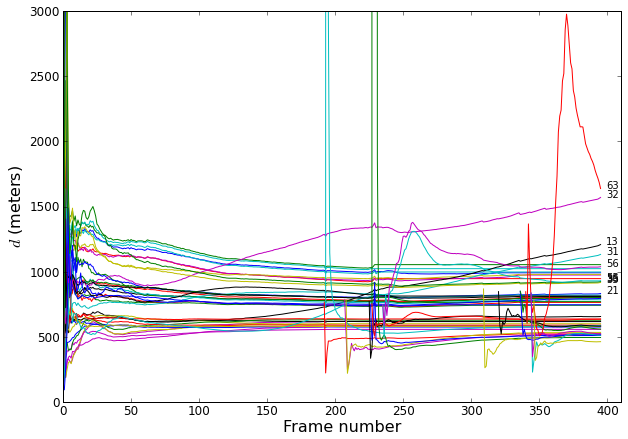
\includegraphics[width=10cm, keepaspectratio=true]
{./Figures/fltfig/cut1/Figure10.png}
\caption{Inverse Depth Convergence}
\label{fltfig:1}
\end{figure}

Although the features initialization point $[x_i, y_i, z_i]$, and the
deviation-elevation angle pair $[\phi, \theta]$ did not go through a
converging stage, they do get updated and converted into the new
camera coordinate using the estimated camera motion at every
iteration. As a result, the accuracy of these parameters varies.
Figure \ref{fltfig:2} shows the tracking of these parameters over 200
frames. These parameters were stable for about 200 frames. Some
features start to drift after 200 frames. This coninside with the
introduction of new feature points into the system. 
% are those featuers that drift are the one that's removed from the
% filter? 
% Does this prove that the filter altered the features parameter
% estimate in order to compensate for the incorrect estimate of the
% UAS localization. Since features removed from the filter were not
% altered for the comppensation, they shows a drift. 
 
\begin{figure}[h]
\centering
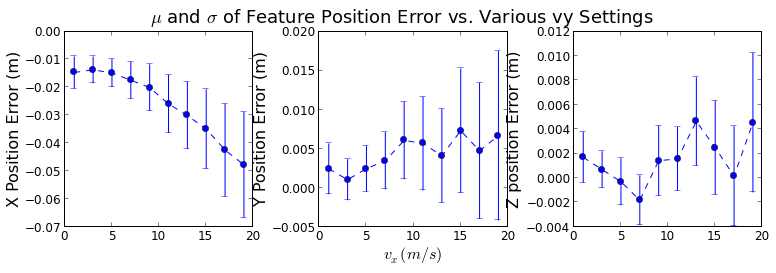
\includegraphics[width=12cm,keepaspectratio=true]
{./Figures/fltfig/cut1/Figure20.jpg}
\caption{Feature paramters (excluding $\rho$)}
\label{fltfig:2}
\end{figure}

Figure 8 illustrate the tracking of feature initialization 
points $[x_{i}, y_{i}, z_{i}]$ in world frame. Ideally, the 
coordinates should converge to a fixed value. However, the plot 
indicates a variation as the vehicle travels along. The plots for xi 
appear to be quite flat because of the large scale of xi value. Figure 9 
shows a more detail xi drift by removing the mean value from the 
recorded sequence. Comparing the pattern of the drift, it is highly 
correlated to the aircraft pitch and yaw rotation (figure?). The 
significant of the drift is measured by the maximum drift seen 
throughout the 200 processed frame, and are listed below (table?). The 
maximum drift is defined by:

Maxdrift = max(abs(initial value - maximum), abs(initial value - 
minimum)) 

\begin{table}[h]
\centering
\begin{tabular}{|l|l|l|}
\hline
Maxmum xi drift & Maximum yi drift & Maximum zi drift \\
\hline
2.21 meters & 18.0...........9 meters & 18.45 meters \\
\hline
\end{tabular}
\end{table}


\begin{figure}[h]
\centering
\includegraphics[width=15.24cm,height=11.44cm]{media/image11.eps}
\end{figure}


\begin{center}Figure 9$x_{i}$ with mean removed\end{center}

Although xi also drifts, its magnitude is significantly less than y and 
z. With maximum drift of 2.2 meters, and mean drift of ?meters, 
considering the magnitude of the initial value for xi, it actually is 
quite stable. 

Converged features

Not converged features

Newly initiated features

\begin{figure}[h]
\centering
\includegraphics[width=15.24cm,height=11.44cm]{media/image12.eps}
\end{figure}


\begin{center}Figure 10 Feature Distance Convergence Plot (1 frame per 
process)\end{center}

\ \ \ \ Figure 10 shows the convergence behavior of inverse depth over 
the 200 frames processed. The plot includes features initialized at 
first frame, as well as those added later on. Features that moved out of 
the field of view of the camera were still kept in the plot, with their 
value kept unchanged. A total of 60 features were initialized and 
tracked. Most features converged to a value within the first 50 frames 
and remained stable. ? features took longer to converge, but started to 
settle in after 120 frames. These features are those on the edge of 
mountain (confirm required).Some other features (? Out of 60) never show 
any convergence behavior. What are these features, and why they don't 
converge?

\begin{figure}[h]
\centering
\includegraphics[width=15.24cm,height=11.44cm]{media/image13.eps}
\end{figure}


\begin{center}Figure 11 plot of angle phi over 200 frames\end{center}

maxdrift\_phi =1.92

\begin{figure}[h]
\centering
\includegraphics[width=15.24cm,height=11.44cm]{media/image14.eps}
\end{figure}


\begin{center}Figure 12 theta plot over 200 frames\end{center}

maxdrift\_theta = 1.5862

\ \ \ \ Figure 11 and 12 shows the tracking of phi and theta over the 
200 frames processed. These two values are calculated from feature 
coordinates on the image plane on the first frame, and should experience 
very little change thereafter. Similar to xi, yi, and zi, value of theta 
and phi is influenced by the aircraft totational motion. The plot of phi 
is highly correlated to aircraft pitch angle, and theta is correlated to 
aircrarft yaw. The change in value for phi and theta is also affected by 
the feature tracking method, and is discussed in detail in section??

\ \ \ \ Another character of SLAM using Kalman filter tracking is that 
the correlation between features grows overtime. This character helps to 
maintain the stability of features parameters during tracking, ie. One 
bad measurement doesn't have big impact on the features parameters. To 
observe whether the examined algorithm carries such character, the 
correlation of the feature parameter: rho, phi, and theta between the 
first feature and all other features are plotted in figure ? All 
parameters are initialized to zero. Over time, all three parameters 
grows to a positive value which indicates a correlation exists between 
features. The correlation for rho decreases over time. For phi, the 
correlation stays unchanged, and for theta, it continues to rise after 
200 frames. 

Newly Initialized features

\begin{figure}[h]
\centering
\includegraphics[width=15.24cm,height=11.44cm]{media/image15.eps}
\end{figure}


\begin{itemize}
\item Covariance between features parameters are initialized to zero
\item Inverse depth covariance converged to a positive number, and then 
decrease slowly as frame number grew.
\item Phi covariance grew to a positive number and remain stable
\item Theta covariance grew to a positive number and continued to 
increase slowly as frame number grew. 
\end{itemize}
\newpage


\subsubsection{Consistency}
Discuss consistency behavior of the state parameters through examining 
of the state covariance matrix. Orientation variance should not decrease 
to zero. If it does, when?

\ \ \ \ In related work, it has been reported that inconsistency occures 
when the UAV travel far away from the origin, and caused the filter to 
diverge. ??? perfomeda analytical analsis on the problem and concluded 
that inconsistency is caused by evalulating the Kalman equations at the 
incorrectly estimated position, instead of the real position. $[$$]$ 
This usually caused the variance of the state vector to decrease, which 
in turn, caused an over confident estimation by the filter. Eventually 
the parameter variance grew to nearly zero, and filter no longer correct 
the state vector using new measurement, and divergence occurs. 

\begin{figure}[h]
\centering
\includegraphics[width=15.24cm,height=11.44cm]{media/image16.eps}
\end{figure}




\begin{figure}[h]
\centering
\includegraphics[width=15.24cm,height=11.44cm]{media/image17.eps}
\end{figure}


\begin{figure}[h]
\centering
\includegraphics[width=15.24cm,height=11.44cm]{media/image18.eps}
\end{figure}




\newpage


\subsubsection{Reliability}
Compare the estimates to ground truth and discuss the accuracy of the 
results

\begin{figure}[h]
\centering
\includegraphics[width=15.24cm,height=11.44cm]{media/image19.eps}
\end{figure}


\begin{center}Figure 13 UAV Flight Path vs. GPS\end{center}

driftUAV = 24.7471 meters

\begin{figure}[h]
\centering
\includegraphics[width=15.24cm,height=11.44cm]{media/image20.eps}
\end{figure}


\begin{center}Figure 14 UAV orientation\end{center}

pitchdrift = -0.7952 degree

yawdrift = 1.2247 degree

\begin{figure}[h]
\centering
\includegraphics[width=15.24cm,height=11.44cm]{media/image21.eps}
\end{figure}


\begin{figure}[h]
\centering
\includegraphics[width=15.24cm,height=11.44cm]{media/image22.eps}
\end{figure}


\begin{figure}[h]
\centering
\includegraphics[width=15.24cm,height=11.44cm]{media/image23.eps}
\caption{\label{figure:_Ref349487278} Z coordinate comparison between 
estimated features and ground truth}
\end{figure}



Because the survey environment is above forestry landscape, there is a 
lack of distinct signature to make visual correspondence between the 
features points and the ground truth map. To make numerical comparison 
between the estimated features positions and the ground truth, some 
assumptions must be made. Based on the observation that feature distance 
is fairly stable once converged, and angle ? is more stable than angle $
\varphi $, the feature coordinate in X and Y is used to find the 
corresponding position in ground truth map, and coordinate in Z is 
compared for accuracy. 

 shows the Z coordinate comparison between the estimated feature and the 
corresponding data point on ground truth map. The estimated feature 
height generally follows the pattern of the ground truth. For features 
located in lower ground, there is a general offset between the estimated 
height and the ground truth. (Need to process a few different pieces to 
identify the error pattern). The statistic on the height error is

Airport Landing Video: (Add another picture circling out the feature 
location in image)

\begin{figure}[h]
\centering
\includegraphics[width=15.24cm,height=7.25cm]{media/image24.eps}
\end{figure}


\begin{figure}[h]
\centering
\includegraphics[width=15.24cm,height=11.37cm]{media/image25.eps}
\end{figure}


Mean Error on X axis = 89.347 meters

Mean Error on Y axis = 119.428 meters

\subsubsection{Impact of the Outliers}
Does the correlation between features help filtering out the outlier 
measurements?

Does the outliers have a negative impact on the overall map quality, and 
how much?

Long term correct measurements help maintaining the system when 
temporary incorrect measurement occurs. Temporary incorrect measurement 
can have a negative impact on the overall map quality. Based on 
properties Consider to delete section

\subsubsection{Use of IMU Improve Vision Tracking Performance in Harsh 
Flight}\label{section:_Toc332876148}
Collect image pairs that shows tracking improvement when using IMU data 
for prediction. Priority: low.

\subsubsection{Variable number of Frame per Process}
\begin{table}[h]
\centering
\begin{tabular}{|l|l|}
\hline
\includegraphics[width=7.83cm,height=5.88cm]{media/image26.eps}
 & \includegraphics[width=7.59cm,height=5.69cm]{media/image27.eps}
 \\
\hline
\includegraphics[width=7.69cm,height=5.77cm]{media/image28.eps}
 & \includegraphics[width=7.66cm,height=5.75cm]{media/image29.eps}
 \\
\hline
\end{tabular}
\end{table}








Feature Height Accuracy

\begin{table}[h]
\centering
\begin{tabular}{|l|l|l|l|l|}
\hline
 & 1 fpp & 2fpp & 3fpp & 4fpp \\
\hline
mean & -6.6648 & -9.6131 & -9.4595 & -8.6598 \\
\hline
std & 36.8959 & 38.9285 & 41.8112 & 45.4366 \\
\hline
max & 86.3177 & 115.2585 & 118.5528 & 132.6752 \\
\hline
min & 0.1958 & 0.0979 & 1.4907 & 0.7791 \\
\hline
\# of features & 60 & 58 & 62 & 60 \\
\hline
\end{tabular}
\end{table}
No advantages seen on the accuracy. Extract feature at the center 
(exclude mountain edge) and re-collect data to see if result shows any 
patter.











Parameters Drift:

\begin{table}[h]
\centering
\begin{tabular}{|l|l|l|l|l|}
\hline
 & 1fpp & 2fpp & 3fpp & 4fpp \\
\hline
xi & 2.2102 & 1.0847 & 0.7589 & 0.6668 \\
\hline
yi & 18.0976 & 12.1789 & 12.4523 & 12.9552 \\
\Hline
zi & 18.4479 & 13.7087 & 8.9254 & 10.5766 \\
\hline
phi & 1.9168 & 1.1715 & 1.2806 (exclude31) & 1.6892 (exclude31,51) \\
\hline
theta & 1.5862 & 1.6326 & 1.6184 (exclude31) & 1.7026 (exclude31,51) \\
\hline
 & & & & \\
\hline
\end{tabular}
\end{table}
Need to check plotting algorithm. Should not have big variation for phi 
and theta plots. 



UAV DRIFT:

\begin{table}[h]
\centering
\begin{tabular}{|l|l|l|l|l|}
\hline
 & 1fpp & 2fpp & 3fpp & 4fpp \\
\hline
GPS & 24.7450 & 19.1648 & 16.8689 & 13.9337 \\
\hline
Pitch & -0.7952 & -1.0177 & -1.2818 & -1.5072 \\
\hline
Yaw & 1.2247 & 1.6169 & 1.8143 & 1.9302 \\
\hline
\end{tabular}
\end{table}
Multiple frames per process improves the UAV translational parameter 
estimation, but offers no advantage in improving the rotational 
parameters drift. 

%%% Local Variables:
%%% mode: latex
%%% TeX-master: "thesis"
%%% End:
